% !TeX encoding = UTF-8
% !TeX spellcheck = hu_HU

\chapter{Monitoring}
\label{chap:monitoring}
\Aref{sect:monitoring}.~alfejezetben ismertetett előnyei miatt a tesztkörnyezetben is egy monitoring rendszer kialakítása mellett döntöttem. Választásom a Prometheus monitorozó rendszerre esett, mely a Grafana vizualizációs eszközzel társítva jó betekintést enged az üzemeltetett rendszerek állapotába. A választásomat az indokolta, hogy ez a párosítás manapság nagyon elterjedt, széles körben használt és jól kibővíthető további adatok monitorozásával, továbbá számos segédanyag áll hozzá rendelkezésre mind a hivatalos oldalon, mind pedig a közösség által karbantartott ismertetők formájában.

\section{Áttekintés}
A továbbiakban tárgyaltak könnyebb megértése végett hasznos megismerni a Prometheus és a kapcsolódó komponensek működését. A Prometheus működési elve egyszerű és hatékony: a figyelt kliensekre úgynevezett \textit{exporter}eket telepítünk, melyeket a Prometheus szerver pull modellt alkalmazva adott időközönként lekérdez. Az exporterek olyan programok, melyek alkalmasak bizonyos statisztikák (pl.~erőforrás-kihasználtság mértéke, adatbázis-lekérdezések gyakorisága) kiolvasására, és ezeket a monitorozott rendszer egy adott portján HTTP-protokollon keresztül közzétenni. Az exporterek önmagukban nem gyűjtenek adatokat, csak adott időközönként frissítik őket, az adatgyűjtést a Prometheus szerver végzi. Figyelt végpontokból rendszerenként több is lehet, mindegyikhez külön-külön port kapcsolódik.

A monitorozás szerves része a riasztások küldése, hiszen a monitoring rendszer folyamatos figyelése nélkül is jó, ha értesülünk a fennálló problémákról, hogy még időben be tudjunk avatkozni. A Prometheus a riasztások kezeléséhez az Alertmanager komponenst kínálja. Ezt részletesen konfigurálhatjuk az igényeinknek megfelelően, hogy milyen típusú problémáról, milyen platformon keresztül és kik kapjanak értesítést. Ez azért is kedvező, mert például egy éles környezet esetében egy alkalmazás összeomlásakor feltehetőleg másnak kell eljárnia, mint amikor hálózati fennakadást (pl.~\acrshort{dns}-probléma\footnote{A~\acrshort{dns} az emberek által könnyen megjegyezhető domain neveket fordítja le az informatikai eszközök által értelmezhető IP-címekre.}) tapasztalunk.

Az összegyűjtött adatokat a Grafana segítségével tehetjük átláthatóbbá, valamint ez teszi könnyebbé a metrikák elemzését is. Adatvizualizációra specializálódott szoftver lévén a Grafana rengeteg opcióval rendelkezik az adatok megjelenítését illetően, így a \acrshort{cpu}-adatok vonalgrafikonon való megjelenítésétől kezdve a szerverünk elérhetőségét jelző igen-nem panelt is választhatunk.
Grafanában a megjelenített adatokat -- melyekhez egy-egy panel tartozik -- úgynevezett \textit{dashboard}okba szervezhetjük. A dashboardok általában összetartozó adatokat tartalmaznak, azaz jó gyakorlat a hardveres erőforrások metrikáit külön dashboardba szervezni például a webszerverhez tartozó mérőszámoktól. % TODO: összesítés dashboard, amin a monitorozott hosztok adatai egy helyen láthatóak?
A Grafana támogatja a Prometheus saját lekérdezőnyelvével, a PromQL-lel való adatszűrést, mely lehetővé teszi a Prometheus szerverrel való egyszerű interakciót.
\Aref{fig:prometheus-architecture}.~ábra egy általános Prometheus-alapú, Grafana adatvizualizációt használó monitoring-architektúrát mutat be.

% tikz ábra beszúrása
\vspace{0.25cm}
\begin{figure}[ht]
	\centering
	\begin{tikzpicture}[node distance=5cm]
	% Define styles
	\tikzstyle{rect} = [rectangle, draw, minimum width=4.2cm, minimum height=2cm, text centered, font=\fontsize{12}{12}\selectfont]
	\tikzstyle{arrow} = [->,>=stealth]
	
	% Nodes
	\node (monitored-host) [rect, rounded corners, align=center, double copy shadow, fill=white] {Monitorozott\\szolgáltatások\\(exporterek)};
	\node (prometheus) [rect, rounded corners, below right of = monitored-host, yshift=-0.5cm] {Prometheus szerver};
	\node (alertmanager) [rect, rounded corners, above right of = prometheus, yshift=0.5cm, align=center] {Prometheus\\Alertmanager};
	\node (grafana) [rect, rounded corners, below of = prometheus, yshift=1cm] {Grafana};
	
	% Arrows
	\draw [arrow] (prometheus) to node[midway, fill=white, inner sep=2pt, align=center] {Metrikák lekérdezése\\(HTTP-kérések)} (monitored-host);
	\draw [arrow] (prometheus) to node[midway, fill=white, inner sep=2pt] {Riasztások} (alertmanager);
	\draw [arrow] (grafana) to node[midway, fill=white, inner sep=2pt] {Adatok lekérdezése} (prometheus);
\end{tikzpicture}

	\caption{A Prometheus monitoring rendszer felépítése~\cite{PrometheusIntro}.}
	\label{fig:prometheus-architecture}
\end{figure}

A Prometheus exporterek egy speciális formátumban teszik közzé az általuk kinyert adatokat. A legegyszerűbb esetben ezek szóközzel elválasztott kulcs-érték párok. Ilyen~adatpárra mutat példát \aref{lst:prometheus-data-format}.~kódrészlet első~sora. A mérőszám elnevezése után kapcsos zárójelekbe szűrőket~(filter) helyezhetünk, ahogy az \aref{lst:prometheus-data-format}.~kódrészlet második~sorában is látható. Lekérdezés esetén az adatokat ugyanezzel a szintaktikával szűrhetjük.
% TODO: lekérdezésre példa

\vspace{2mm}
\begin{lstlisting}[caption=Prometheus exporterek által közzétett adatok.,label=lst:prometheus-data-format, numbers=left]
	node_load1 0.35
	node_hwmon_temp_celsius{chip="platform_coretemp_1",sensor="temp2"} 28
\end{lstlisting}

\section{Telepítés, konfiguráció}
\label{sect:monitoring-installation}
A környezet beüzemelését nagyban segítette, hogy a Prometheus monitoring rendszert az Uyuni külön Salt~Formulákon keresztül támogatja. Így lehetőség van az infrastruktúra-menedzsment rendszerbe bevont klienseken manuális csomagtelepítés nélkül egy kezdetleges monitoring környezetet kialakítani. Ez a gyakorlatban azt jelentette, hogy az Uyuni a beállított Formulák alapján a kliensekre telepítette az alapvető rendszer-információkat lekérdező \textit{Node exportert}, míg a monitoring szerveren egy alapbeállításokkal rendelkező Prometheus szervert és a hozzá kapcsolódó Grafana szervert telepítette.

% TODO: nagyobb betűméret a képen
\begin{figure}[ht]
	\centering
	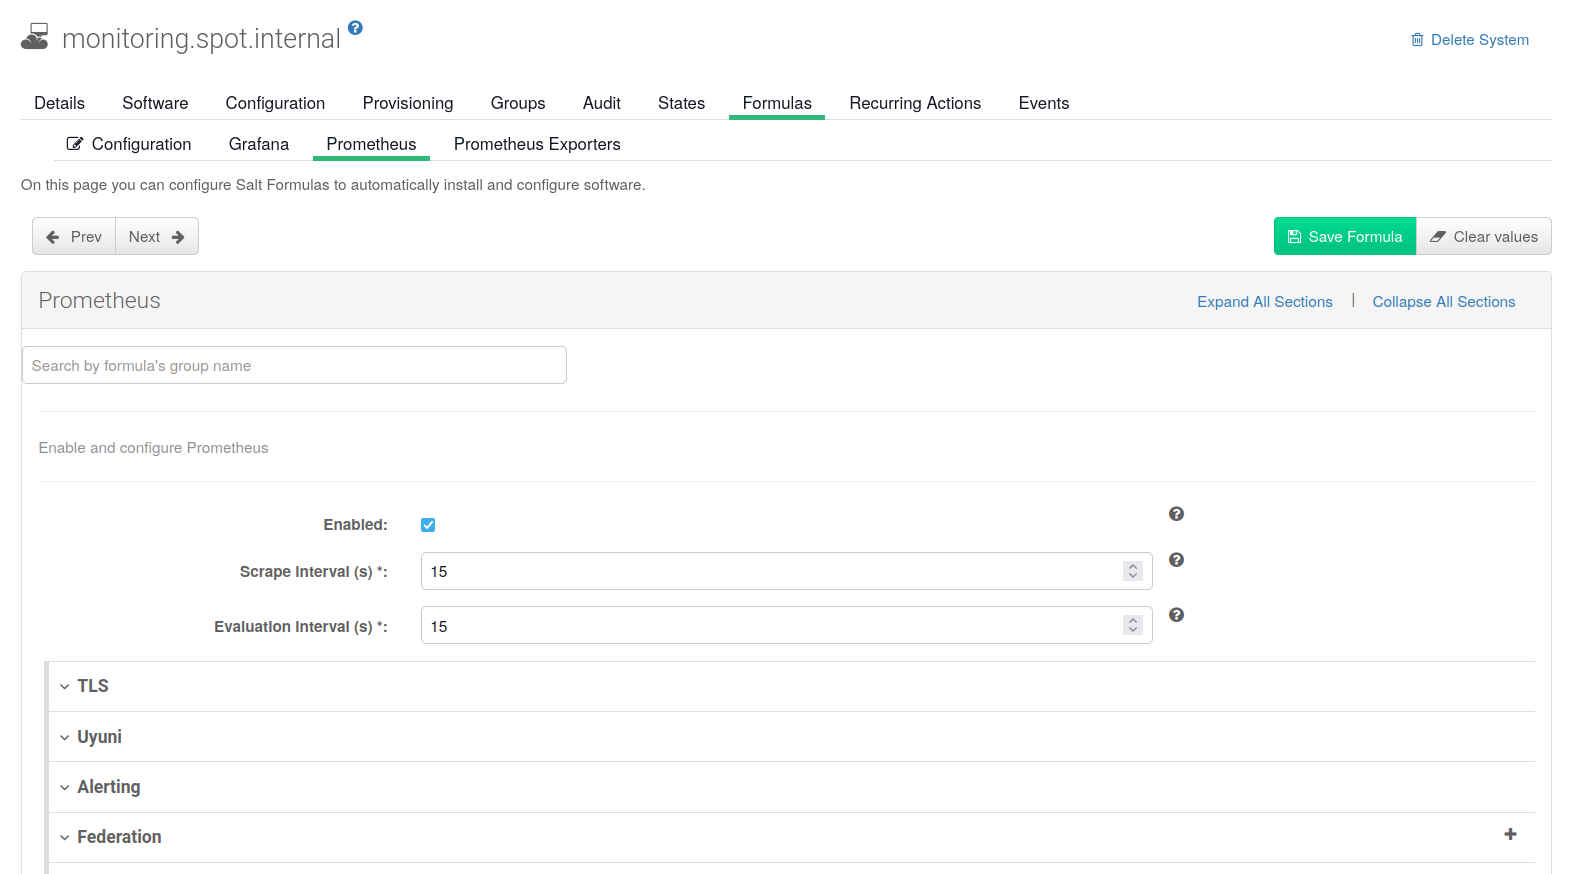
\includegraphics[width=15cm]{figures/prometheus-formula.png}
	\caption{Az Uyuni webes felületéről könnyen módosíthatjuk a Prometheus szerver alapvető beállításait.}
	\label{fig:prometheus-formula}
\end{figure}

\subsection{Konténerhoszt monitorozása}
A monitoring rendszer kialakítása során nehézséget jelentett, hogy openSUSE Leap Micro-ra nem volt hivatalosan elérhető a felügyelt gépekről hardver- és kernelstatisztikákat szolgáltató Node exporter szoftvercsomag formájában. Emiatt eleinte a konténerhoszt monitorozására nem volt lehetőségem. A megoldást az jelentette, hogy az exportert egy konténerben telepítettem a virtuális gépre. Mivel a konténer azonban a gazdagéptől elkülönülten fut, ezért módosítani kellett a konténer futtatásához használt parancsot. A~\texttt{--path.rootfs=/host} kapcsoló beállításával az exporter már a konténerből is képes volt elérni a gazdagép metrikáit, így ezt a hosztot is sikerült bevonni a monitoring rendszerbe.

\subsection{Tűzfal beállítása}
Az operációs rendszerek telepítése során a tűzfal engedélyezését választottam. Ez azt jelentette, hogy szinte minden port zárva volt a külvilág felé, így a Prometheus szerver sem tudta elérni az exporterek által szolgáltatott adatokat.

Ahhoz, hogy a monitoring rendszer az elvárt módon működjön, szükséges volt a tűzfalszabályok módosítása. A telepített rendszereken a \texttt{firewalld} az alapértelmezett tűzfal, melynek a beállításait a \texttt{firewall-cmd} segédprogram segítségével tudtam módosítani~(\ref{lst:firewalld-add-port}.~kódrészlet első~sora). A kódrészlet harmadik sorában a szükséges portok kinyitását követő állapot látható az Uyunit futtató szerver esetében, a monitoring rendszerben használt exportereket, rövid leírásukat és a kapcsolódó portszámokat \aref{tab:monitoring-exporters}.~táblázat tartalmazza. A monitoring szerverhez tartozó Salt~Formula alkalmazásával automatikusan települ a Tomcat és Taskomatic exporter. Ezek az Uyuni alapjait adó webes keretrendszerről és a használt feladatütemezőről biztosítanak statisztikákat.

\vspace{2mm}
\begin{lstlisting}[caption=Tűzfalszabályok módosítása.,label=lst:firewalld-add-port, numbers=left,escapechar=?]
	?\underline{uyuni:$\sim$ \#}? firewall-cmd --permanent --add-port=9117/tcp
	?\underline{uyuni:$\sim$ \#}? firewall-cmd --list-ports
	5556/tcp 5557/tcp 9100/tcp 9117/tcp 9187/tcp 9800/tcp
\end{lstlisting}

\begin{table}[h]
	\setlength{\tabcolsep}{5pt}
	\renewcommand{\arraystretch}{1.3}
	\centering
	\begin{tabular}{||l l m{7.6cm}||}
		\hline
		Portszám & Exporter & Leírás \\
		\hline\hline
		5556 & Tomcat JMX exporter & Az Uyuni működéséhez szükséges Tomcat alkalmazás Java-processzéről jelenít meg adatokat (pl.~szálak, memóriahasználat). \\
		\hline
		5557 & Taskomatic JMX exporter & Az Uyuni által használt Tascomatic alkalmazás Java-processzéről jelenít meg adatokat (pl.~szálak, memóriahasználat). \\
		\hline
		9090 & Prometheus exporter & A Prometheus állapotáról tesz közzé adatokat (pl.~hibás lekérések száma, lekérések mérete).  \\
		\hline
		9100 & Node exporter & Linux hosztokról publikál számos hardver- és kernelmetrikát (pl.~erőforrás-használat, kontextusváltások). \\
		\hline
		9117 & Apache exporter & Az Apache webszerverről ad meg mérőszámokat (pl.~egyes HTTP-státuszkódokhoz tartozó lekérdezések száma, \acrshort{cpu}-idő).  \\
		\hline
		9187 & PostgreSQL exporter & Az Uyuni által használt PostgreSQL adatbázismotorról oszt meg adatokat (pl.~zárak száma, rekordlekérdezési és frissítési ráta).  \\
		\hline
		9800 & Taskomatic exporter & Az Uyuni által használt Taskomatic feladatütemező metrikáit jeleníti meg (pl.~elvégzett feladatok száma, aktuális szálak száma).  \\
		\hline
	\end{tabular}
	\caption{A monitoring rendszerben használt Prometheus exporterek a hozzájuk tartozó portszámokkal.}
	\label{tab:monitoring-exporters}
\end{table}

% tikz ábra beszúrása
\begin{figure}[ht]
	\centering
	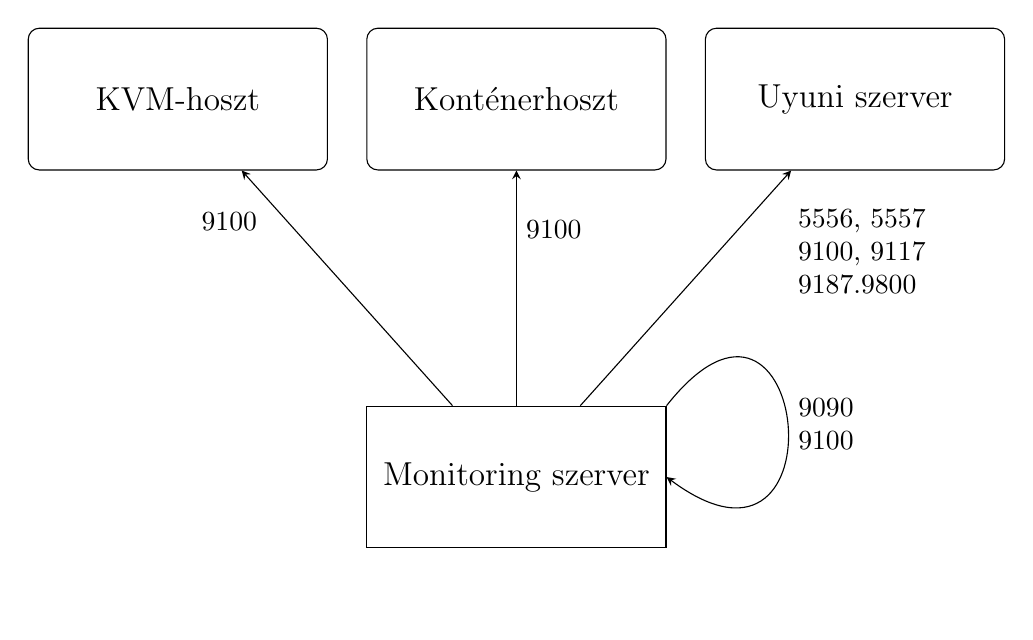
\begin{tikzpicture}[node distance=4.3cm]
	\tikzstyle{rect} = [rectangle, draw, minimum width=3.8cm, minimum height=1.8cm, text centered, font=\fontsize{12}{12}\selectfont]
	\tikzstyle{arrow} = [->,>=stealth]
	
	\node (kvm) [rect, rounded corners] {KVM-hoszt};
	\node (containers) [rect, rounded corners, right of = kvm] {Konténerhoszt};
	\node (uyuni) [rect, rounded corners, right of = containers] {Uyuni szerver};
	\node (monitoring) [rect, below of = containers, yshift=-0.5cm] {Monitoring szerver};
	
	\draw [arrow] (monitoring) to node[above left, near end, xshift=-10, yshift=-4, align=left] {9100} (kvm);
	\draw [arrow] (monitoring) to node[near end, right] {9100} (containers);
	\draw [arrow] (monitoring) to node[near end, right, align=left, xshift=18, yshift=-8] {5556, 5557\\9100, 9117\\9187.9800} (uyuni);
	\draw [arrow, loop, bend left] (monitoring.north east) to[out=150, in=60, looseness=8, align=left, xshift=3] node[right] {9090\\9100} (monitoring.east);
\end{tikzpicture}

	\caption{A monitoring rendszerbe bevont gépek a rajtuk futó exporterek által használt portokkal.}
	\label{fig:monitoring-setup}
\end{figure}

\section{Riasztások beállítása}
A Prometheus-alapú monitoring rendszer egyik legfontosabb komponense az Alertmanager, hiszen ennek segítségével a gyűjtött adatok folyamatos szemmel tartása nélkül is értesülhetünk a rendszerünket érintő lényeges eseményekről.
\Aref{fig:prometheus-architecture}.~ábrán látható, hogy az Alertmanager egy különálló modul a monitoring-infrastruktúrában. Ez a modularitás a gyakorlatban is megjelenik: az Alertmanager a Prometheustól elkülönülten, a~\texttt{golang-github-prometheus-alertmanager} csomaggal telepíthető, a telepítést követően pedig egy külön konfigurációs fájl és systemd unit fájl tartozik hozzá, azaz a Prometheus adatgyűjtő részétől elkülönülten kezelhető.

A tesztkörnyezetben az Alertmanager konfigurációját Salt state-tel végeztem. Ehhez létrehoztam egy új konfigurációs csatornát (configuration channel, \ref{fig:alertmanager-state}.~ábra), mely tartalmazta az Alertmanager konfigurációs állományát, valamint az ennek érvényre jutását biztosító state fájlt.

% TODO: kép nagyítása
\begin{figure}
	\centering
	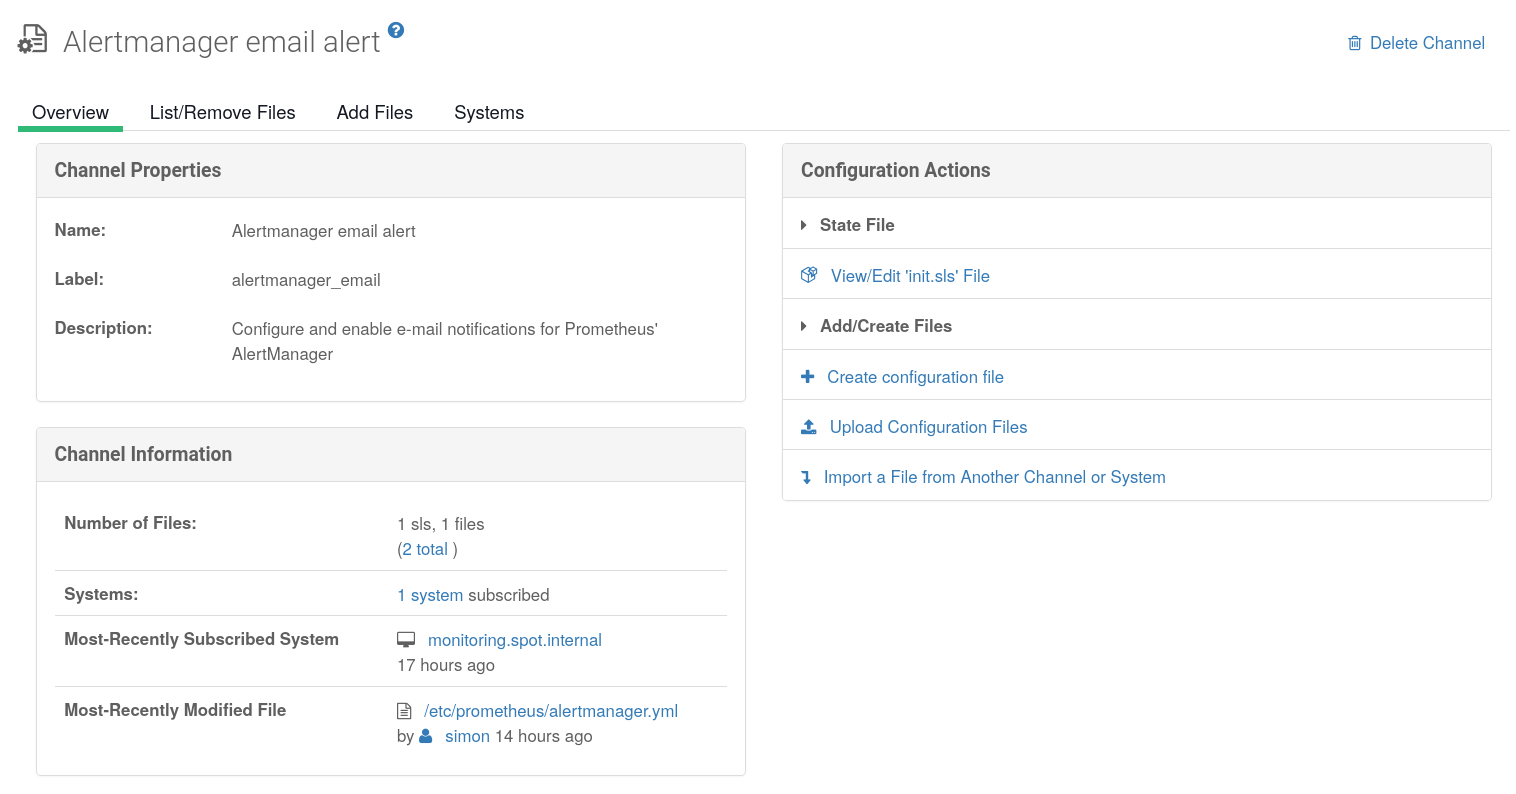
\includegraphics[width=15cm]{figures/alertmanager-state.png}
	\caption{A monitoring értesítések kezeléséhez használt Salt state.}
	\label{fig:alertmanager-state}
\end{figure}

A riasztáskezelő alrendszer beállításának célja az volt, hogy egy monitorozott szolgáltatás elérhetetlenné válása esetén az azt figyelő rendszer küldjön értesítést e-mailben a hibáról. Ennek megvalósításához \aref{lst:alertmanager-yml-short}.~kódrészleten látható beállításokat használtam. Itt megfigyelhető a lokális \acrshort{smtp}-szerver megadása, és az értesítések küldéséhez használt e-mail cím beállítása.
Az 5.~sorban kezdődő \texttt{route} beállítás adja meg, hogy a specifikusabb szűrőkre nem illeszkedő riasztásokkal hogy járjunk el. Ebben az esetben ezeket csoportosítjuk a riasztás típusa és az azt küldő hoszt alapján. A \texttt{receivers} címkén belül adhatjuk meg, hogy a riasztásokat milyen végpontokra küldje a rendszer. A konfigurációs fájlban szereplő beállítások egy egyszerű e-mailt küldenek a megadott címre. Mivel a~titkosítás használata a lokális gépen futó levelezőszerver esetében nem indokolt, és konfigurációja összetett, ezért a 13.~sorban látható \texttt{require\_tls} opcióval ezt kikapcsoltam. Fontos azonban, hogy ezt csak helyi mail szerver esetén tehetjük meg, amennyiben egy központi levelezőszervert használunk, akkor a program nem is engedi a titkosítás kikapcsolását~\cite{PrometheusAlertmanagerConfig}.
A 14.~sorban látható \texttt{send\_resolved} opciót igazra állítva a szolgáltatások helyreállásáról is kapunk értesítést. % TODO: példa riasztás email?
A teljes, kommentekkel ellátott konfigurációs fájlt a~\nameref{cha:appendix}~\ref{lst:alertmanager-config-full}.~kódrészlete tartalmazza.


% TODO: oldaltörés javítása?
% TODO: a teljes kódrészlet legyen a függelékben
% https://tex.stackexchange.com/a/224743
\begin{figure}[htb]
	\lstinputlisting[caption=Az e-mail-értesítések küldéséhez használt konfigurációs fájl részlete.,label=lst:alertmanager-yml-short, numbers=left]{listings/alertmanager.yml.short}
\end{figure}

A fent ismertetett konfigurációs fájlt \aref{lst:alertmanager-state}.~kódrészleten szereplő Salt state-tel telepítettem a monitoring szerverre. Ehhez a Salt által fájlok kezelésére nyújtott \texttt{file.managed} state opciót használtam, majd a kódrészlet 4.~sorában szereplő \texttt{source} címkével megadtam az Uyuni által kezelt leírófájlt, valamint beállítottam a telepítendő fájl elérési útját és a kapcsolódó jogosultságokat (\ref{lst:alertmanager-state}.~kódrészlet 5-7.~sora). 
A Salt-tal való konfiguráció-menedzsment a \texttt{service.running} state opcióval lehetőséget kínál a kapcsolódó service újratöltésére, amit a \texttt{watch} opció beállításával automatikusan is megtehetünk. Így tehát a kódrészlet 16.~sorában megadott fájl módosulása esetén az alertmanager-t futtató systemd service automatikusan újraindításra kerül a módosítások érvényre juttatásával, ezzel is csökkentve a manuális beavatkozás szükségességét.

\begin{figure}[ht]
	\lstinputlisting[caption=Az e-mail-értesítések beállítását végző konfigurációs állomány telepítéséhez használt Salt state.,label=lst:alertmanager-state, numbers=left]{listings/alertmanager-init.sls}
\end{figure}


\section{Adatvizualizáció}
A gyűjtött adatok áttekintése, elemzése segítségünkre lehet további rendszerek telepítése során például szükséges erőforrások mennyiségének becsléséhez, illetve szolgáltatáskiesést követően segíthet a probléma meghatározásában.

\Aref{sect:monitoring-installation}.~alfejezetben ismertetettek alapján a tesztkörnyezetben a Grafana adatvizualizációs eszközt használtam. Ez jó integrációt biztosít a Prometheushoz, könnyen lekérdezhetőek a különböző metrikák. A telepítéshez használt Salt~Formula pedig még egyszerűbbé tette a Grafana használatát: az alapértelmezett konfigurációs fájl számos előre definiált, a rendszerek állapotát jól összefoglaló dashboardot tartalmaz, így a tűzfalbeállításon és néhány panel webes felületen történő személyre szabásán túl nem volt szükséges részletesebben konfigurálni.

\Aref{fig:grafana-uyuni-server}.~ábrán látható dashboard az Uyuni szerver állapotát ismerteti. Ez a dashboard is a Grafana Salt Formula része, néhány panel mértékegységének pontosításán és skálázásán kívül nem volt szükség a beállítások módosítására. Az ilyen nézetek előnye, hogy segítségükkel nagyon hamar megállapíthatjuk a rendszereink állapotát, hiszen minden lényeges mérőszámot tartalmaznak: segítségével figyelemmel követhetjük például a rendszer terheltségét, a processzor és a memória kihasználtságát, a hálózat- és háttértárhasználat rátáját, az adatbázis-műveletek állapotát és a háttértárak kihasználtságát.

\begin{figure}[ht]
	\centering
	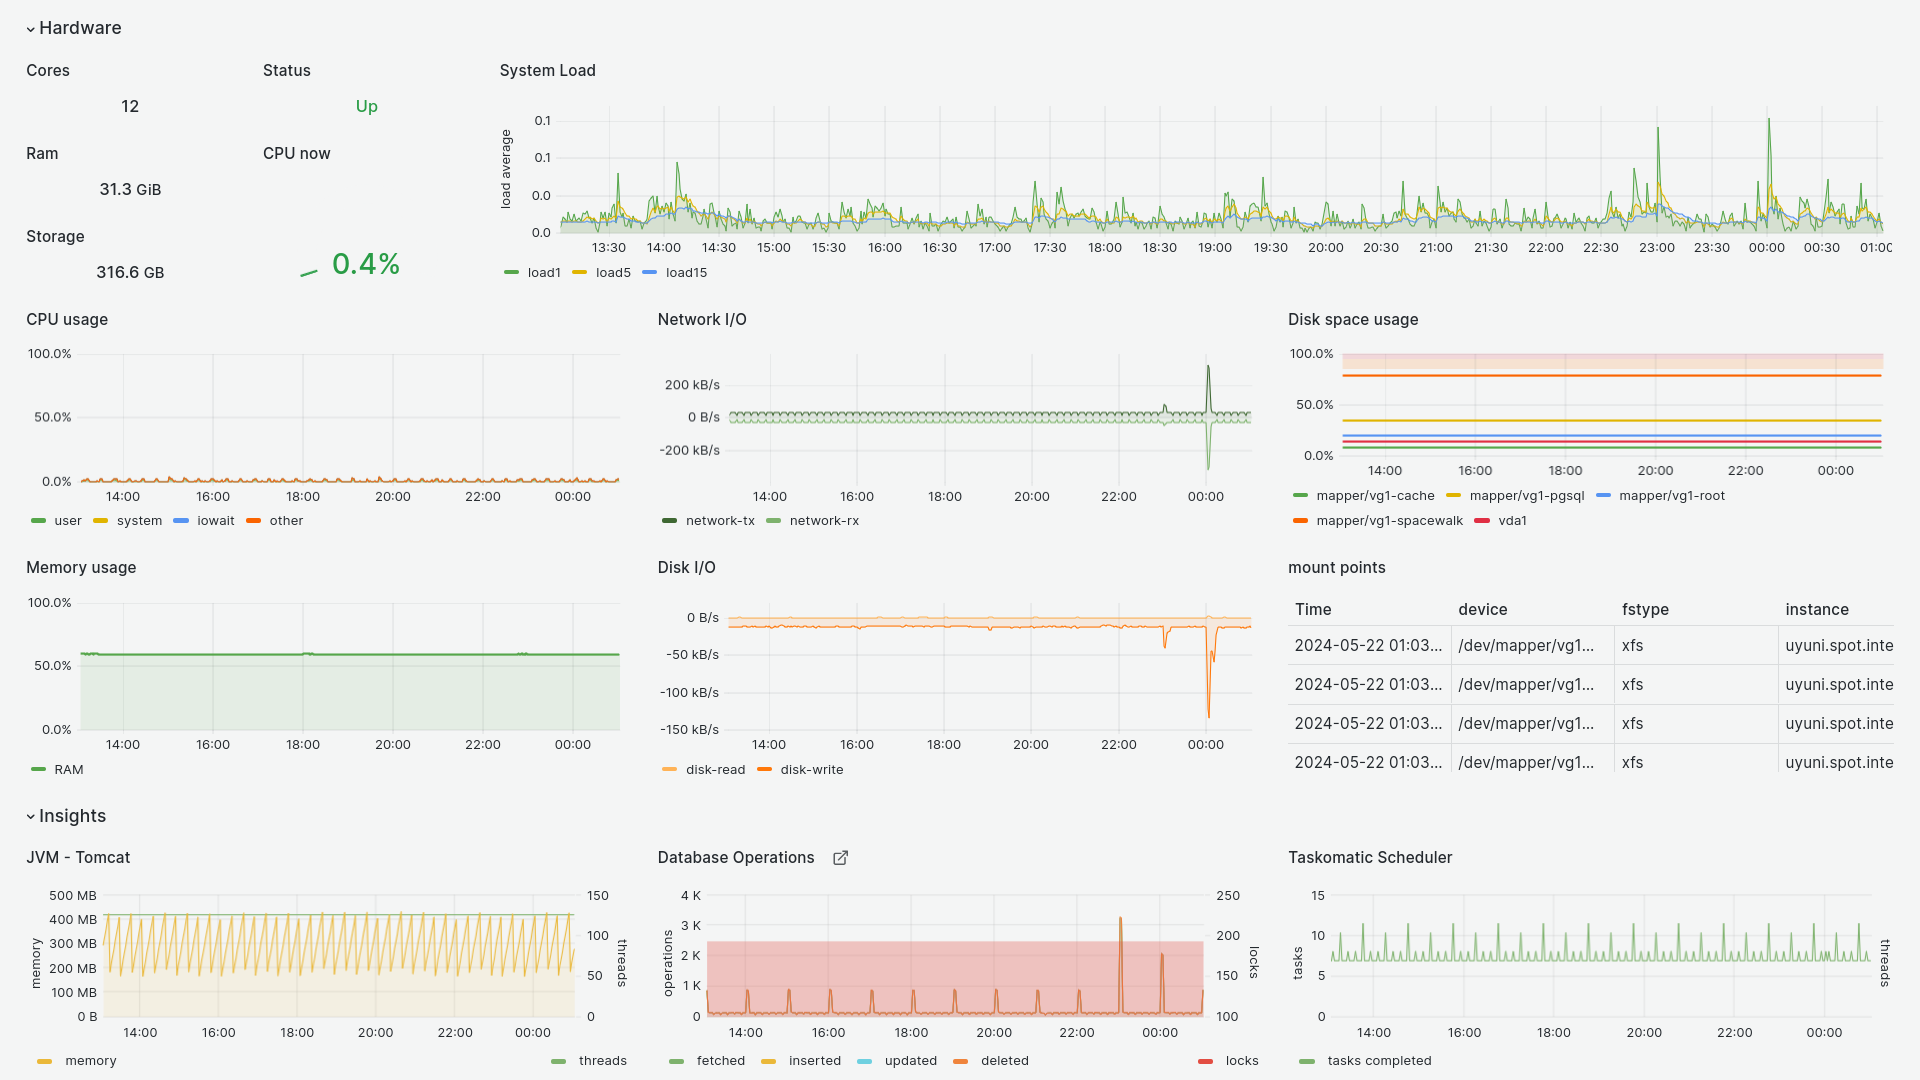
\includegraphics[width=15cm]{figures/grafana-uyuni-server.png}
	\caption{A tesztkörnyezetben használt Grafana egyik dashboardja az Uyuni szerver fontosabb mérőszámait mutatja be.}
	\label{fig:grafana-uyuni-server}
\end{figure}

% TODO: két-két és fél számmal?
Bár a tesztkörnyezet körülbelül két-két és fél hónapos folyamatos üzemeltetése során nem voltak jelentős kimaradások, az Uyuni kezdetleges konfigurációja során az egyik telepítőforrás tükrözése során többször is leállt az azt futtató gép, így valós helyzetben nyílt alkalmam a metrikák visszanézésére, és a hiba okának felkutatására. Az incidens során megjelenő grafikont \aref{fig:reboot-grafana}.~ábra mutatja be. A grafikon jobb oldalán látható a négy leállás, a bal szélén pedig láthatjuk, hogy néhány órával korábban hasonlóan magas terhelés mellett nem lépett fel a hiba. A grafikon $ y $ tengelyén láthatjuk, hogy az nem 100\%-ig, hanem sokkal tovább fut. Ennek oka, hogy a rendszerterhelés számítása során az egy processzormagra eső maximális terhelést tekintjük a 100\%-nak, így egy 24~\acrshort{cpu}-val rendelkező gép esetén a maximális érték 2400\% lenne. A grafikonon 1600\%~körülre esik a legnagyobb terhelés, ami összhangban van az Uyunit futtató virtuális gép által maximálisan használható 16~processzormaggal. Mint később kiderült, a hibát hardveres hiba okozta, a virtuális gép által használható processzormagok csökkentésével a probléma nem jelentkezett többé.

\begin{figure}[h!t]
	\centering
	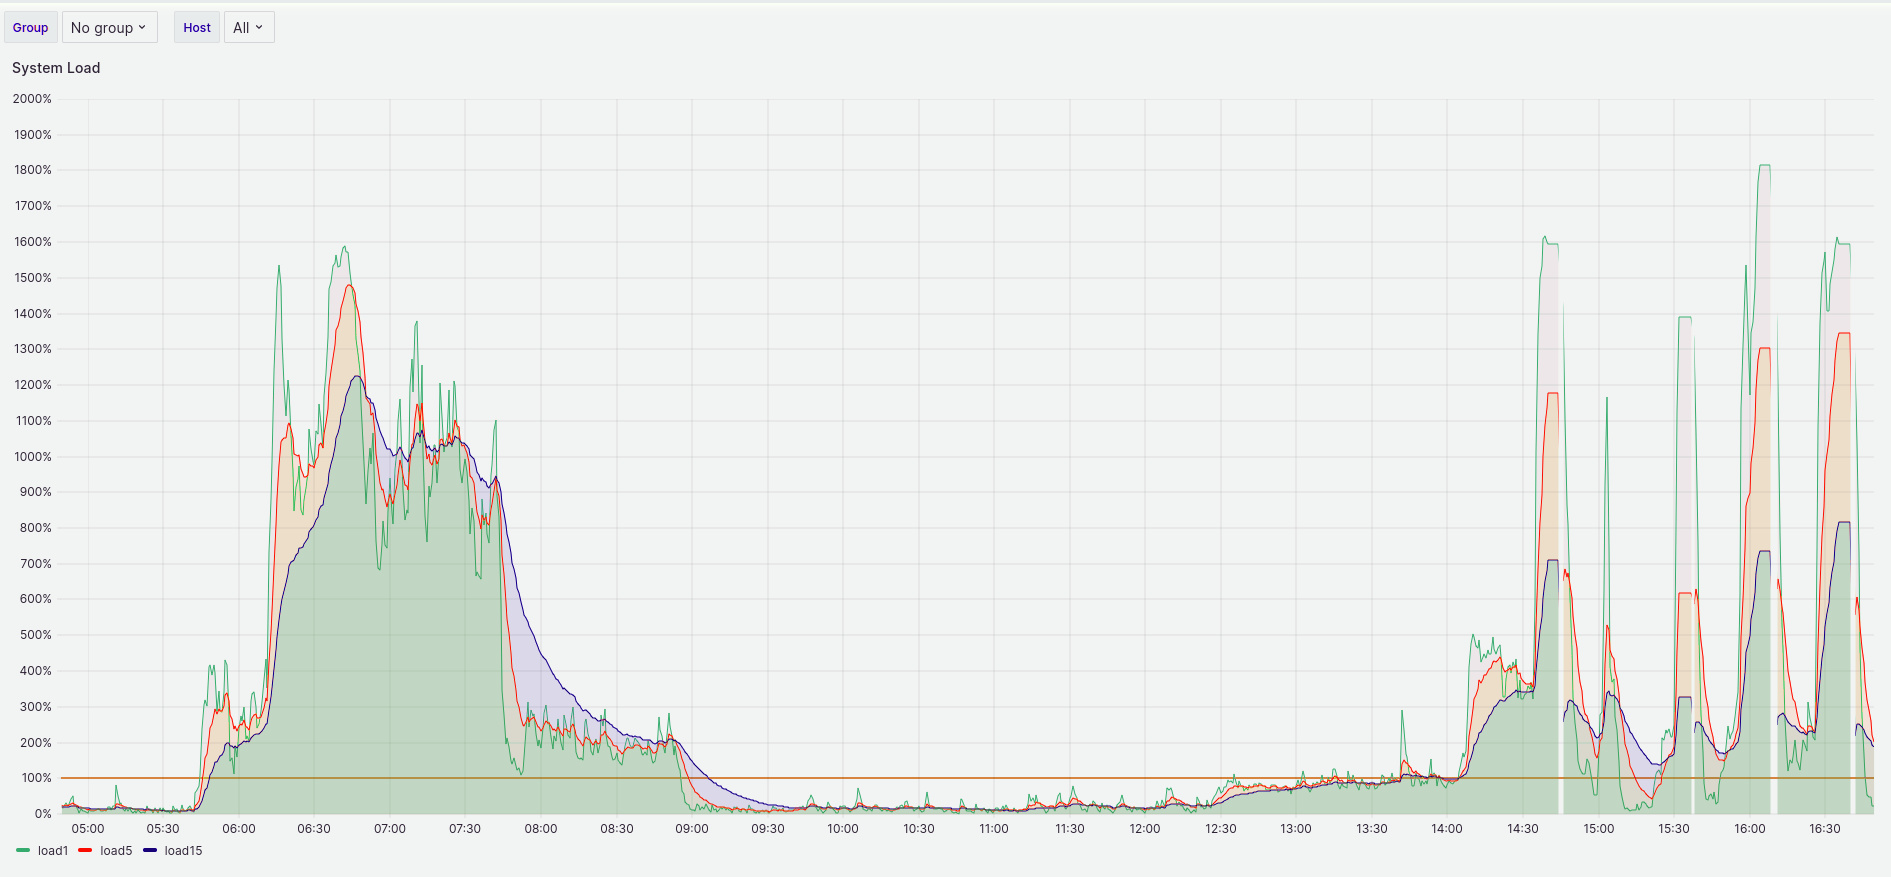
\includegraphics[width=15cm]{figures/reboot-grafana-invert.jpg}
	\caption{A telepítőforrás-tükrözés során tapasztalt szolgáltatáskiesések a Grafanaban megjelenő grafikonon. Az ábrán a~rendszer terheltsége látható az idő függvényében.}
	\label{fig:reboot-grafana}
\end{figure}
